\documentclass{article}

% packages
\usepackage{amsmath, amsthm, thmtools, amsfonts, amssymb, luacode, catchfile, tikzducks, hyperref, ifthen}
\ifcsname c@kobocompile\endcsname
	\usepackage[a5paper, total={1072pt, 1448pt}, margin=10pt, includeheadfoot]{geometry} % set page margins
\else
	\usepackage[a4paper, margin=50pt, includeheadfoot]{geometry}
\fi
\usepackage[shortlabels]{enumitem}
\usepackage[skip=3pt, indent=0pt]{parskip}

% language
\usepackage[bidi=basic, layout=tabular, provide=*]{babel}
\ifcsname c@english\endcsname
	\babelprovide[main, import]{english}
\else
	\babelprovide[main, import]{hebrew}
	\babelprovide{rl}
\fi
%\babelfont{rm}{Libertinus Serif}
\babelfont{rm}[Renderer=Harfbuzz]{Libertinus Serif}
\babelfont{sf}{Libertinus Sans}
\babelfont{tt}{Libertinus Mono}

% style
\AddToHook{cmd/section/before}{\clearpage}	% Add line break before section
\linespread{1.3}
\setcounter{secnumdepth}{0}		% Remove default number tags from sections, this won't do well with theorems
\AtBeginDocument{\setlength{\belowdisplayskip}{3pt}}
\AtBeginDocument{\setlength{\abovedisplayskip}{3pt}}
\graphicspath{ {../images/} }

% operators
\DeclareMathOperator\cis{cis}
\DeclareMathOperator\Sp{Sp}
\DeclareMathOperator\tr{tr}
\DeclareMathOperator\im{Im}
\DeclareMathOperator\re{Re}
\DeclareMathOperator\diag{diag}
\DeclareMathOperator*\lowlim{\underline{lim}}
\DeclareMathOperator*\uplim{\overline{lim}}
\DeclareMathOperator\rng{rng}
\DeclareMathOperator\Sym{Sym}
\DeclareMathOperator\Arg{Arg}
\DeclareMathOperator\Log{Log}
\DeclareMathOperator\dom{dom}
\DeclareMathOperator\supp{Supp}
\DeclareMathOperator\var{Var}
\DeclareMathOperator\cov{Cov}

% commands
%\renewcommand\qedsymbol{\textbf{מש''ל}}
%\renewcommand\qedsymbol{\fbox{\emoji{lizard}}}
\newcommand{\Aa}[0]{\mathcal{A}}
\newcommand{\Bb}[0]{\mathcal{B}}
\newcommand{\CC}[0]{\mathbb{C}}
\newcommand{\Cc}[0]{\mathcal{C}}
\newcommand{\EE}[0]{\mathbb{E}}
\newcommand{\FF}[0]{\mathbb{F}}
\newcommand{\Ff}[0]{\mathcal{F}}
\newcommand{\Ii}[0]{\mathcal{I}}
\newcommand{\Gg}[0]{\mathcal{G}}
\newcommand{\Ll}[0]{\mathcal{L}}
\newcommand{\Mm}[0]{\mathcal{M}}
\newcommand{\NN}[0]{\mathbb{N}}
\newcommand{\Nn}[0]{\mathcal{N}}
\newcommand{\PP}[0]{\mathbb{P}}
\newcommand{\Pp}[0]{\mathcal{P}}
\newcommand{\QQ}[0]{\mathbb{Q}}
\newcommand{\RR}[0]{\mathbb{R}}
\newcommand{\Rr}[0]{\mathcal{R}}
\newcommand{\Ss}[0]{\mathcal{S}}
\newcommand{\TT}[0]{\mathbb{T}}
\newcommand{\Uu}[0]{\mathcal{U}}
\newcommand{\Vv}[0]{\mathcal{V}}
\newcommand{\Ww}[0]{\mathcal{W}}
\newcommand{\ZZ}[0]{\mathbb{Z}}
\newcommand{\acts}[0]{\circlearrowright}
\newcommand{\explain}[2] {
	\begin{flalign*}
		 && \text{#2} && \text{#1}
	\end{flalign*}
}
\newcommand{\maketitleprint}[0]{ \begin{center}
	%\begin{tikzpicture}[scale=3]
	%	\duck[graduate=gray!20!black, tassel=red!70!black]
	%\end{tikzpicture}	
	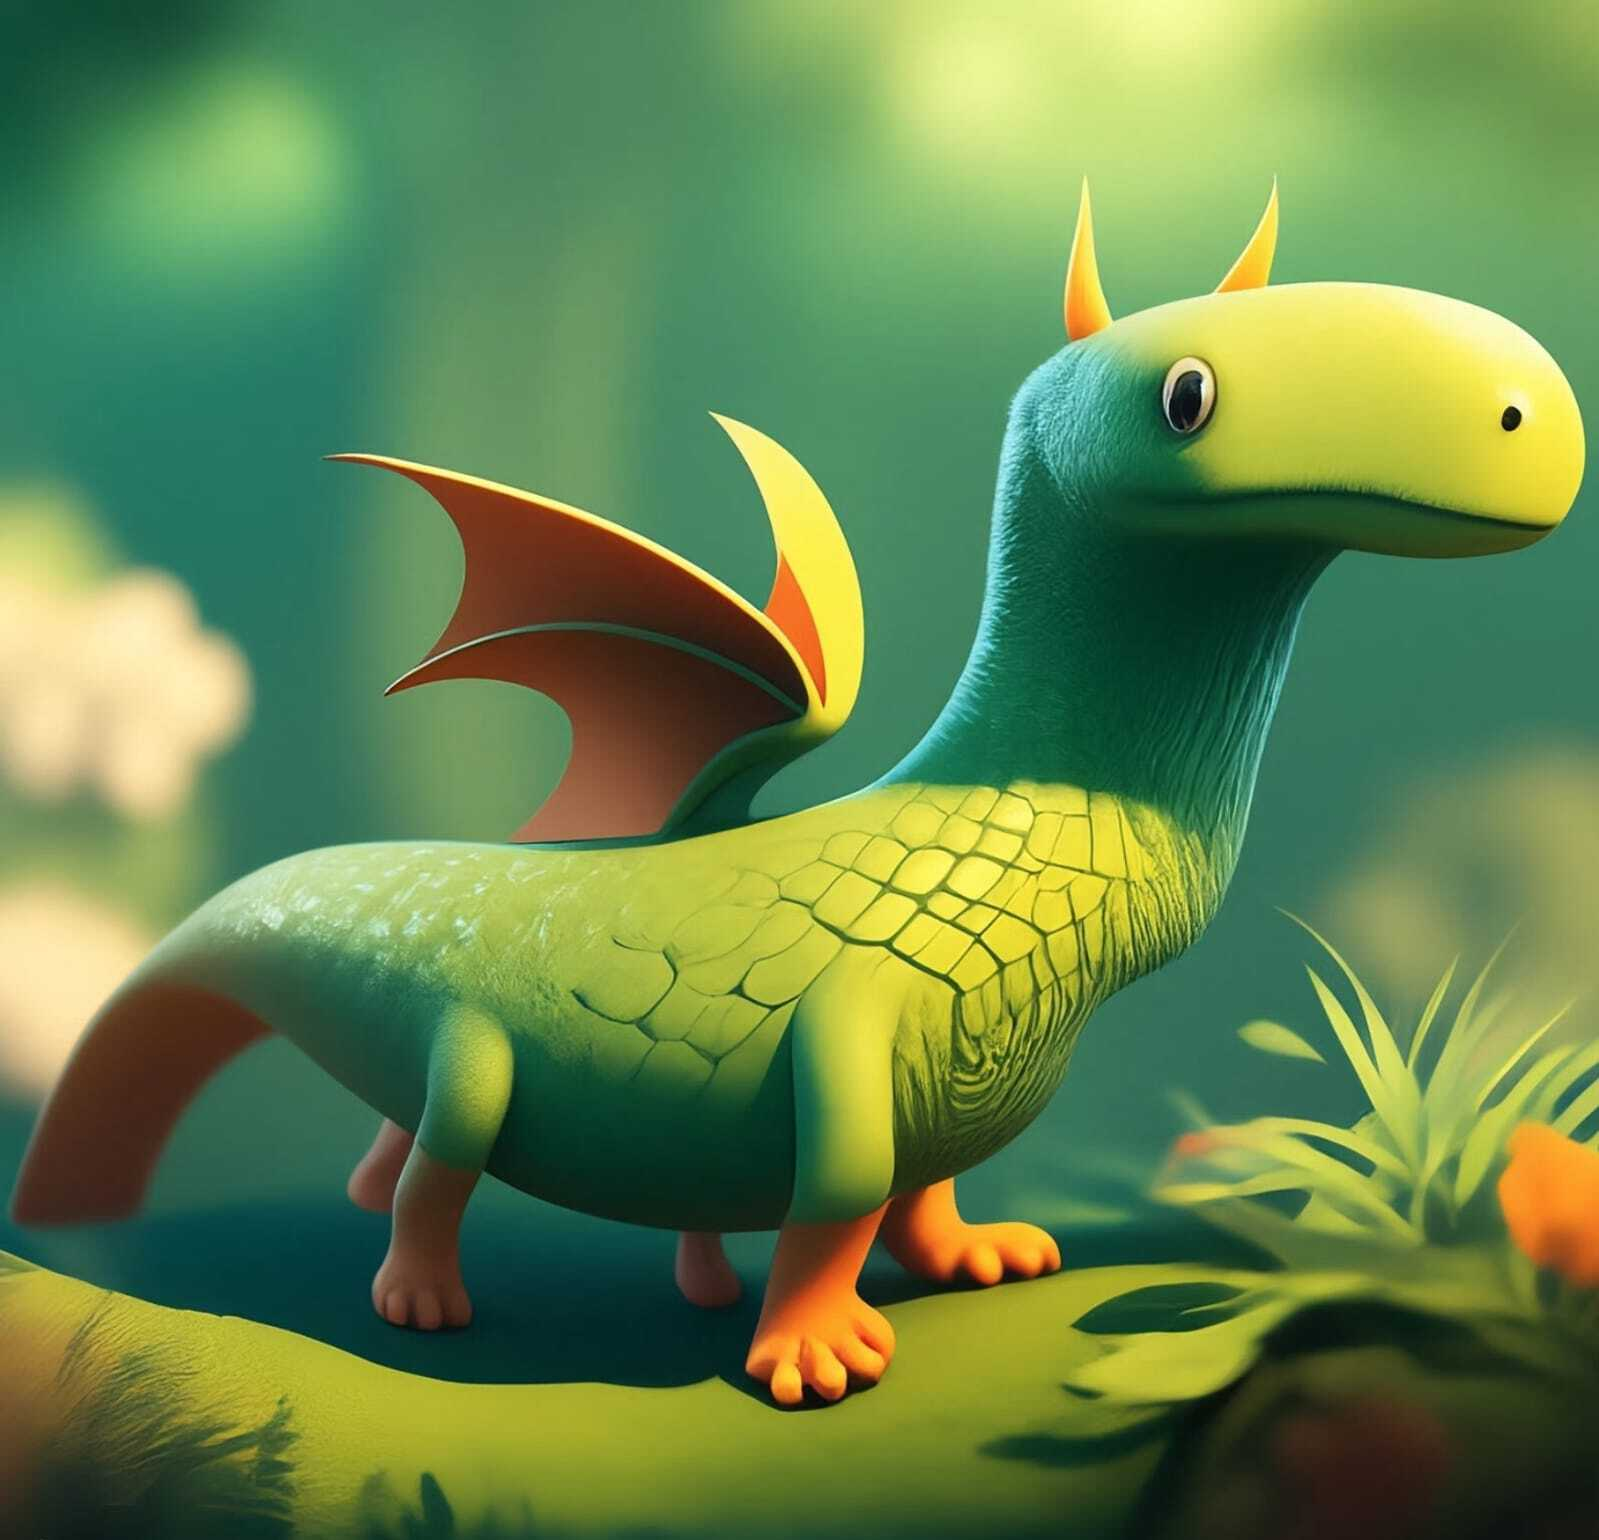
\includegraphics[width=6cm]{cover}
\end{center}
}

% theorem commands
\newtheoremstyle{c_remark}
	{}	% Space above
	{}	% Space below
	{}% Body font
	{}	% Indent amount
	{\bfseries}	% Theorem head font
	{}	% Punctuation after theorem head
	{.5em}	% Space after theorem head
	{\thmname{#1}\thmnumber{ #2}\thmnote{ \normalfont{\text{(#3)}}}}	% head content
\newtheoremstyle{c_definition}
	{3pt}	% Space above
	{3pt}	% Space below
	{}% Body font
	{}	% Indent amount
	{\bfseries}	% Theorem head font
	{}	% Punctuation after theorem head
	{.5em}	% Space after theorem head
	{\thmname{#1}\thmnumber{ #2}\thmnote{ \normalfont{\text{(#3)}}}}	% head content
\newtheoremstyle{c_plain}
	{3pt}	% Space above
	{3pt}	% Space below
	{\itshape}% Body font
	{}	% Indent amount
	{\bfseries}	% Theorem head font
	{}	% Punctuation after theorem head
	{.5em}	% Space after theorem head
	{\thmname{#1}\thmnumber{ #2}\thmnote{ \text{(#3)}}}	% head content

\ifcsname c@english\endcsname
	\theoremstyle{plain}
	\newtheorem{theorem}{Theorem}[section]
	\newtheorem{lemma}[theorem]{Lemma}
	\newtheorem{proposition}[theorem]{Proposition}
	\newtheorem*{proposition*}{Proposition}
	%\newtheorem{corollary}[theorem]{אין חלופה עברית}

	\theoremstyle{definition}
	\newtheorem{definition}[theorem]{Definition}
	\newtheorem*{definition*}{Definition}
	\newtheorem{example}{Example}[section]
	\newtheorem{exercise}{Exercise}[section]

	\theoremstyle{remark}
	\newtheorem*{remark}{Remark}
	\newtheorem*{solution}{Solution}
	\newtheorem{conclusion}[theorem]{Conclusion}
	\newtheorem{notation}[theorem]{Notation}
\else
	\theoremstyle{c_plain}
	\newtheorem{theorem}{משפט}[section]
	\newtheorem{lemma}[theorem]{למה}
	\newtheorem{proposition}[theorem]{טענה}
	\newtheorem*{proposition*}{טענה}
	%\newtheorem{corollary}[theorem]{אין חלופה עברית}

	\theoremstyle{c_definition}
	\newtheorem{definition}[theorem]{הגדרה}
	\newtheorem*{definition*}{הגדרה}
	\newtheorem{example}{דוגמה}[section]
	\newtheorem{exercise}{תרגיל}[section]

	\theoremstyle{c_remark}
	\newtheorem*{remark}{הערה}
	\newtheorem*{solution}{פתרון}
	\newtheorem{conclusion}[theorem]{מסקנה}
	\newtheorem{notation}[theorem]{סימון}
\fi

% Questions related commands
\newcounter{question}
\setcounter{question}{1}
\newcounter{sub_question}
\setcounter{sub_question}{1}

\ifcsname c@english\endcsname
	\newcommand{\question}[1][0]{
		\ifthenelse{#1 = 0}{}{\setcounter{question}{#1}}
		\section{Question \arabic{question}}
		\addtocounter{question}{1}
		\setcounter{sub_question}{1}
	}

	\newcommand{\subquestion}[1][0]{
		\ifthenelse{#1 = 0}{}{\setcounter{sub_question}{#1}}
		\subsection{Part \alph{sub_question}}
		\addtocounter{sub_question}{1}
	}
\else
	\newcommand{\question}[1][0]{
		\ifthenelse{#1 = 0}{}{\setcounter{question}{#1}}
		\section{שאלה \arabic{question}}
		\addtocounter{question}{1}
		\setcounter{sub_question}{1}
	}

	\newcommand{\subquestion}[1][0]{
		\ifthenelse{#1 = 0}{}{\setcounter{sub_question}{#1}}
		\subsection{סעיף \localecounter{letters.gershayim}{sub_question}}
		\addtocounter{sub_question}{1}
	}
\fi

% import lua and start of document
\directlua{common = require ('../common')}

\GetEnv{AUTHOR}

% headers
\author{\AUTHOR}
\date\today

\title{פתרון מטלה מסכמת --- אנליזה על יריעות, 80426}
% chktex-file 17
% chktex-file 9

\DeclareMathOperator{\vol}{vol}
\DeclareMathOperator{\Div}{div}

\begin{document}
\maketitle
\maketitleprint[blue]

\question{}
נתאר את הוכחת משפט הדיברגנץ ליריעות קומפקטיות עם שפה.
\begin{proof}
	בגרסה ללא השפה האסטרטגיה הייתה בנייה של זרימה מתאימה לשדה הווקטורי הנתון $X$ על־ידי שימוש בזרימה מקומית וקומפקטיות.
	לבסוף על־ידי שימוש במשפט הווריאציה הראשונה נוכל לקבל שקילות לאינטגרל על הדיברגנץ, היא מקבעת את ערכו לאפס.

	עתה נתאר את משפט הדיברגנץ עצמו, ניסוח המשפט הוא חלק משמעותי בהוכחתו, והוא נכתב כעת מתוך התפיסה שיש לזכור אותו בדיוק.
	תהי $M^k \subseteq \RR^n$ יריעה קומפקטית עם שפה.
	נניח גם ש־$X : M \to \RR^n$ שדה וקטורי משיק ל־$M$, כלומר ש־$X(p) \in T_p(M)$ לכל $p \in M$.
	אז מתקיים,
	\[
		\int_M \Div_M X\ d\vol_k
		= \int_{\partial M} \langle X(p), \nu(p) \rangle\ d\vol_{k - 1}(p)
	\]
	כלומר ערך האינטגרל הוא ערך האינטגרל בשפה של מכפלה בנורמל חיצוני, שלא במפתיע אין תלות בשפה (ולמעשה כבר עתה יכולנו להוכיח זאת ישירות מחלוקת היריעה לשפתה ולפנימה), והתלות היא בכמה היריעה התרחבה בתהליך $X$.

	לאחר הבנה מעמיקה של המשפט, נוכל להסביר את הוכחתו, היא כיאה לכל משפט רציני מתחילה ברדוקציות.
	הרדוקציה הראשונה מטרתה לגרוס כי השדה הווקטורי הוא מכווץ בלבד, כלומר,
	\[
		\langle X(p), \nu(p) \rangle < 0
	\]
	ונוכל להשיג אותו על־ידי שימוש בקומפקטיות ובמציאת מקסימום של $X$ על השפה $\partial M$, נוכל לבנות יריעה חדשה שמזיזה את $X$ פנימה בלבד, ונעשה זאת ככה שנוכל לחשב את האינטגרל בקלות ובהתאם לקבל את הרדוקציה.

	עתה נגיע לחלק הבא, שלב הבניות.
	המטרה שלנו היא לפרק את $M$ בדרך הנוחה ביותר, ונעשה זאת על־ידי הגדרת ''משיכת שפה'', כלומר נגדיר את הזרימה החד־צדדית שמובטח לנו שקיימת, ונגדיר את היריעה $N_t = \varphi([0, t] \times \partial M)$.
	המפתח בשלב זה עבורי הוא תפיסה טובה של משמעות $N_t$, וכאמור ניתן לתאר אותו כמשיכה ש־$\varphi$ מבצעת על השפה, נוכל לדמיין זאת על־ידי סימון השפה ביריעה, הפעלת $\varphi$ ובדיקת המיקומים שהשפה עוברת בהם.
	מבנה זה מאפשר לנו לבצע את הפירוק (עד כדי חיתוך ממידה אפס),
	\[
		M = \varphi_t(M) \cup N_t
	\]
	ובהתאם לטענה האחרונה, נוכל גם להסיק,
	\[
		\vol_k(M)
		= \vol_k(\varphi_t(M)) + \vol_k(N_t)
	\]
	אם נגזור את הביטוי נקבל אם כך,
	\[
		0 = 
		\left. \frac{d}{dt} \vol_k(\varphi_t(M)) \right\lvert_{t = 0}
		+ \left. \frac{d}{dt} \vol_k(N_t) \right\lvert_{t = 0}
	\]
	ועל־ידי שימוש שקול לגרסה ללא שפה במשפט הווריאציה הראשונה גם,
	\[
		\int_M \Div_M(X)\ d\vol_k
		= - \left. \frac{d}{dt} \vol_k(N_t) \right\lvert_{t = 0}
	\]
	כלומר עלינו לנתח את $N_t$ בלבד כדי למצוא את הטענה.
	אבל ישירות מהגדרת $N_t$ אנו יודעים כי (ופוביני),
	\[
		\vol_k(N_t)
		= \int_{\partial M} \int_{0}^{t} V(D \varphi |_{(x, s)})\ ds\ d\vol_{k - 1}(x)
	\]
	מהמשפט היסודי של החשבון האינפיניטסימלי נוכל להסיק שגם,
	\[
		- \frac{d}{dt} \left. \vol_k(N_t) \right\lvert_{t = 0}
		= \int_{\partial M} V(D \varphi |_{(x, 0)})\ d\vol_{k - 1}(x)
	\]
	כלומר המשפט כולו שקול לטענה שמתקיים,
	\[
		V(D \varphi |_{(x, 0)}) = - \langle X(x), \nu(x) \rangle
	\]
	טענה זו נובעת משימוש בהוכחה סטנדרטית של בחירת בסיס ושימוש באפיון השקול של אופרטור נפח וברדוקציה הראשונה.
\end{proof}
הוכחה זו כתובה כך שהחלקים שניתנים להשלמה עבורי הושמטו, כל מה שנכתב הוא מה שהייתי כותב גם במפתח הוכחה עבור שינונה לקראת מבחן.

\question{}
\subquestion{}
נוכיח את משפט הפונקציה ההפוכה לנקודות שפה. \\
תהינה $M \subseteq \RR^m, N \subseteq \RR^n$ יריעות עם שפה.
נניח גם ש־$f : M \to N$ העתקה חלקה כך ש־$f(\partial M) \subseteq \partial N$.
נסמן $p \in \partial M$ ו־$q \in \partial N$ נקודות כך ש־$f(p) = q$ ו־$D f |_p : T_p M \to T_q N$ איזומורפיזם לינארי. \\
נראה שקיימות סביבות פתוחות $p \in U \subseteq M$ ו־$q \in V \subseteq N$ כך ש־$f |_U : U \to V$ היא דיפאומורפיזם.
\begin{proof}
	תהי $\alpha : U_0 \to \alpha(U_0)$ פרמטריזציה מקומית של $p \in U_0 \subseteq \HH^k$ ב־$M$ עבור $k = \dim M$.
	נניח ש־$\beta : V_0 \to \alpha(V_0)$ פרמטריזציה מקומית של $q \in V_0 \subseteq \HH^k$ ב־$N$.
	אם $f^{-1}(V_0) \subseteq U_0$ אז נגדיר $U = f^{-1}(V_0)$ ו־$V = V_0$, על־ידי שימוש באפיון של רציפות.
	אחרת $U = f^{-1}(V_0) \cap U_0$ היא קבוצה פתוחה 

	נניח בלי הגבלת הכלליות ש־$\alpha(0) = p, \beta(0) = q$, זאת שכן נוכל לבצע הזזות וכן מהעובדה שהוכחה במהלך הקורס שמתקיים,
	\[
		\alpha(({\{ 0 \}}^{k - 1} \times \RR) \cap U_0) \subseteq \partial M
	\]
	אז $U_0 \cap V_0$ היא קבוצה פתוחה ונסמן,
	\[
		U = \alpha(U_0 \cap V_0),
		\quad
		V = \beta(U_0 \cap V_0)
	\]
	כל פרמטריזציה מקומית היא דיפאומורפיזם ולכן הומיאומורפיזם ובהתאם העתקה פתוחה, לכן $U \subseteq M, V \subseteq N$ קבוצות פתוחות.
	עתה נגדיר את $g : U_0 \cap V_0 \to \HH^k$ על־ידי,
	\[
		g = \beta \circ f \circ \alpha^{-1}
	\]
	אז בהכרח $g$ רגולרית ב־$(0, 0)$ מהנתונים, והיא הפיכה בסביבה פתוחה של הראשית על־ידי שימוש במשפט מאינפי 3 והרחבה רציפה של $g$.
	נניח ש־$0 \in U' \subseteq U_0 \cap V_0$ סביבה כזו, אז נוכל לצמצם את $U, V$ בהתאם ל־$\alpha^{-1}(U')$ ו־$\beta^{-1}(g(U'))$.
\end{proof}

\subquestion{}
נניח ש־$M^k \subseteq \RR^n$ יריעה ללא שפה,
ותהי $U \subseteq \RR^k$ פתוחה כלשהי.
נניח ש־$\alpha : U \to M$ היא חלקה כך ש־$D \alpha |_x$  מדרגה $k$ לכל $x \in U$. \\
נראה ש־$\alpha$ היא העתקה פתוחה.
\begin{proof}
	עבור נקודה כלשהי $x \in U$ מהנתון $\alpha$ רגולרית ב־$x$ ולכן ממשפט הפונקציה ההפיכה $\alpha |_V : V \to \alpha(V)$ היא דיפאומורפיזם הפיך, כאשר $x \in V \subseteq U$ פתוחה.
	אבל טענה זו נכונה לכל $x$, כלומר $\alpha$ הפיכה מקומית בכל מקום, ולכן הפיכה ובהתאם גם דיפאומורפיזם ולכן בפרט הומיאומורפיזם ומאפיון שקול העתקה פתוחה.
\end{proof}

\subquestion{}
בהגדרה של יריעות פתוחות פרמטריזציה דורשת את תנאי הפתיחות, אבל בסעיף הקודם מצאנו שפתיחות נובעת מקיום העתקה חלקה לסביבה של היריעה.
אנו נסביר עתה את הקשר שבין שתי הטענות הלכאורה מעט סותרות הללו.
\begin{solution}
	בהוכחת הטענה כבר התבססנו על תכונת הפתיחות המקומית של היריעה, למעשה הטענה שראינו בסעיף ב' היא דרך מצוינת להבין מה היא יריעה.
	כלומר, נוכל להסיק שיריעה מתנהגת באופן מספיר ''יפה'' כדי לאפשר לפונקציות רגולריות להיות גם פתוחות באופן ישיר, ובכך הן האובייקט שקושר בין דיפאומורפיזם (ובפרט הומיאומורפיזם ופתיחות) לבין קבוצה במרחב.
\end{solution}

\question{}
נסמן ב־$C$ את מעגל היחידה במישור $xy$ ב־$\RR^3$, כלומר $C = \partial \{ (x, y, 0) \in \RR^3 \mid x^2 + y^2 = 1 \}$,
ונסמן גם את הפרמטריזציה שלו,
\[
	\gamma(t)
	= (\cos t, \sin t, 0)
\]
נגדיר את השדה הווקטורי $F$ על $\RR^3 \setminus C$ המוגדר על־ידי,
\[
	F(x)
	= \int_{0}^{2 \pi} \frac{x - \gamma(t)}{{\lVert x - \gamma(t) \rVert}^3} \times  \gamma'(t)\ dt
\]
כאשר,
\[
	{(u_1, u_2, u_3)}^t \times {(v_1, v_2, v_3)}^t
	= {(u_2 v_3 - u_3 v_2, u_3 v_1 - u_1 v_3, u_1 v_2 - u_2 v_1)}^t
\]
וכאשר האינטגרל מבוצע קורדינטה־קורדינטה.

\subquestion{}
נראה ש־$F$ הוא משמר מקומית.
\begin{proof}
	תהי $p \in \RR^3$, נגדיר ${\{ e_i \}}_{i = 1}^3 \subseteq \RR^3$ הבסיס הסטנדרטי של המרחב, ונחשב,
	\begin{align*}
		\nabla {\lVert x - p \rVert}^{-1}
		& = \nabla {\left(\sum_{i = 1}^3 {(x_i - p_i)}^2 \right)}^{-1/2} \\
		& = \sum_{j = 1}^3 - \frac{1}{2} \cdot 2 (x_j - p_j) \cdot {\left(\sum_{i = 1}^3 {(x_i - p_i)}^2 \right)}^{-3/2} e_j \\
		& = \sum_{j = 1}^3 \frac{p_j - x_j}{{\lVert x - p \rVert}^3} e_j \\
		& = \frac{p - x}{{\lVert x - p \rVert}^3}
	\end{align*}
	נבחין גם כי,
	\begin{align*}
		(x - \gamma(t)) \times \gamma'(t)
		& = (x - (\cos t, \sin t, 0)) \times (- \sin t, \cos t, 0) \\
		& = (- x_3 \cos t, - x_3 \sin t, (x_1 - \cos t) \cos t + (x_2 - \sin t) \sin t) \\
		& = (- x_3 \cos t, - x_3 \sin t, x_1 \cos t + x_2 \sin t - 1)
	\end{align*}
	אנו רוצים להראות שימור מקומי, כלומר שמתקיים,
	\[
		\frac{\partial F_i}{\partial x_i}
		= \frac{\partial F_j}{\partial x_j}
	\]
	לכל $i, j \in [3]$.
	אבל,
	\[
		F(x)
		= \int_{0}^{2 \pi} (\nabla {\lVert x - \gamma(t) \rVert}^{-1}) \times \gamma'(t)\ dt
	\]
	אם נסמן $g(x) = {\lVert x - \gamma(t) \rVert}^{-1}$ אז נקבל,
	\[
		(- \frac{\partial g}{\partial x_3} \cos t, - \frac{\partial g}{\partial x_3} \sin t, 
	.\]
\end{proof}

\end{document}
